\documentclass[11pt, a4paper, english]{book}

\usepackage{unir}

\usepackage{apacite}
\usepackage{caption}
\usepackage{eso-pic}
\usepackage{float}
\usepackage{graphicx}
\usepackage{minted}
\usepackage[nottoc]{tocbibind}
\usepackage{picture}
\usepackage{subcaption}

\hypersetup{
  colorlinks = true, % Colors links instead of ugly boxes
  urlcolor   = azulunir, % Color for external hyperlinks
  linkcolor  = azulunir, % Color of internal links
  citecolor  = azulunir, % Color of citations
}

% Bibliography style
\bibliographystyle{apacite}

\setlength{\headheight}{15pt}

%---------------------------
% Título del trabajo y autor
%---------------------------
\title{Open Clusters Characterization in Gaia DR2 Using ML Algorithms}
\author{Carlos David Álvaro Yunta}
\date{12th of November, 2020}
\director{César Augusto Guzmán Álvarez}
\nombreciudad{Madrid, Spain}

%---------------------------
%marges
%---------------------------
%\usepackage[margin=1.9cm]{geometry}
%---------------------------
%---------------------------
%---------------------------
%---------------------------
\begin{document}
%\renewcommand{\listfigurename}{Índice de Ilustraciones}
%\renewcommand{\listtablename}{Índice de Tablas}
%\renewcommand{\contentsname}{Índice de Contenidos}
%\renewcommand{\figurename}{Figura}
%\renewcommand{\tablename}{Tabla}

\maketitle

\frontmatter
\tableofcontents
\listoffigures
\listoftables

\chapter{Abstract}

{\bf Nota:} En este apartado se introducirá un breve resumen en inglés del trabajo realizado (extensión máxima: 150 palabras).
Este resumen debe incluir el objetivo o propósito de la investigación, la metodología, los resultados y las conclusiones.

\medskip

{\bf Key words.} open clusters detection --- machine learning --- gaia dr2 --- data analysis

\chapter{Resumen}

{\bf Nota:} En este apartado se introducirá un breve resumen en español del trabajo realizado (extensión máxima: 150 palabras).
Este resumen debe incluir el objetivo o propósito de la investigación, la metodología, los resultados y las conclusiones.

\medskip

{\bf Palabras Clave:} detección de cúmulos abiertos --- inteligencia artificial --- gaia dr2 --- análisis de datos

\chapter{Acknowledgement}

This work has made use of data from the European Space Agency (ESA) mission
{\it Gaia} (\url{https://www.cosmos.esa.int/gaia}), processed by the {\it Gaia}
Data Processing and Analysis Consortium (DPAC,
\url{https://www.cosmos.esa.int/web/gaia/dpac/consortium}). Funding for the DPAC
has been provided by national institutions, in particular the institutions
participating in the {\it Gaia} Multilateral Agreement.

\medskip

This publication makes use of VOSA, developed under the Spanish Virtual Observatory project
supported by the Spanish MINECO through grant AyA2017-84089.
VOSA has been partially updated by using funding from the European Union's Horizon 2020 Research
and Innovation Programme, under Grant Agreement nº 776403 (EXOPLANETS-A)

\medskip

This research has made use of the VizieR catalogue access tool, CDS, Strasbourg, France (DOI : 10.26093/cds/vizier).
The original description of the VizieR service was published in 2000, \cite[A\&AS 143, 23]{ochsenbein2000vizier}

\mainmatter
\chapter{Introduction}

% TODO: 1.1 Motivation

% ¿Cuál es el problema a tratar?
% ¿Cuáles crees que son las causas?
% ¿Por qué es relevante el problema?

% TODO: 1.2 Planteamiento

% ¿Cómo se podría solucionar el problema?
% ¿Qué es lo que se propone?
% Descripción del objetivo del trabajo en términos generales

% TODO: 1.3 Estructura de la memoria

% Descripción breve de lo que se va a contar en cada uno de los capítulos siguientes.

Stellar open clusters (OC) \cite{janes1982open} are groups of stars gravitationally bound originated from a single molecular gas cloud.
Thus they share the same chemical composition and age, and they have similar relative positions and proper motion.
These astronomical objects are of fundamental importance to understand the spiral structure,
the dynamics and the chemical evolution of our galaxy.

Although most stars in the Milky Way are presented isolated, it is considered that most of them (or even all)
are formed in clustered environments and spend a period of time gravitationally bound with their siblings embedded
in their original molecular cloud
\cite{clarke2000theformationofstellarclusters} \cite{portegies2010young}.
The evolution of these systems tends to sparse them in a few million years by interacting gravitationally with other systems.
Galactic tidal forces and mechanisms that involves the gas loss driven by stellar feedback are other causes of disruption
\cite{brinkmann2017bound}.
Nevertheless, a small fraction of these systems will survive in the initial state and persist bound in bigger timescales.

Young OC allow us to research stars formation regions and improve our understanding about the mechanisms that create those stars.
On the other side, older OC give us information about stellar processes and how the galactic disk evolves.
Some highly disturbed orbits could also provide evidence of recent merge events and accretion traces from outside the galaxy
\cite{cantat2016abundances}.

The study of OC has been pushed forward thanks to the huge and precise dataset from the Gaia mission
\cite{collaboration2016description} Gaia DR2 \cite{gaia2018gaia}, available since 2018.
This dataset has helped to review already known open clusters and to find new ones.

Stars that belong to a same OC share relative positions, so their parallax value is similar among them. They also share similar values of
proper motion, both in right ascension and declination. Another property, since these stars were born from the same gas cloud and at the same
temporary stage, their metallicity must be uniform. However, to take into account this last property, we face the inconvinient that this
parameter is not directly available in Gaia DR2 database. We will avoid this issue by looking at $E(b-r) / G_{mag}$ diagrams with well
defined isochrone curves \cite{bressan2012parsec}. These isochrone curves are derived from theoretical models that mainly involve metallicity
and mass/brightness from stars. With these models we can define important properties for the development of stars and their evolution in the
H-R diagram. Examples of these curves are shown in Figure \ref{fig:examples_of_isochrones}.

Again, since these stars were born close in time, regarding their intrinsic properties (mass/brightness), these stars must present a very
well defined and sharp profile with low sparsing through the main sequence in the H-R diagram.

We will take advantage of these properties to validate that the open clusters obtained are right.

\begin{figure}[htbp]
  \centering
  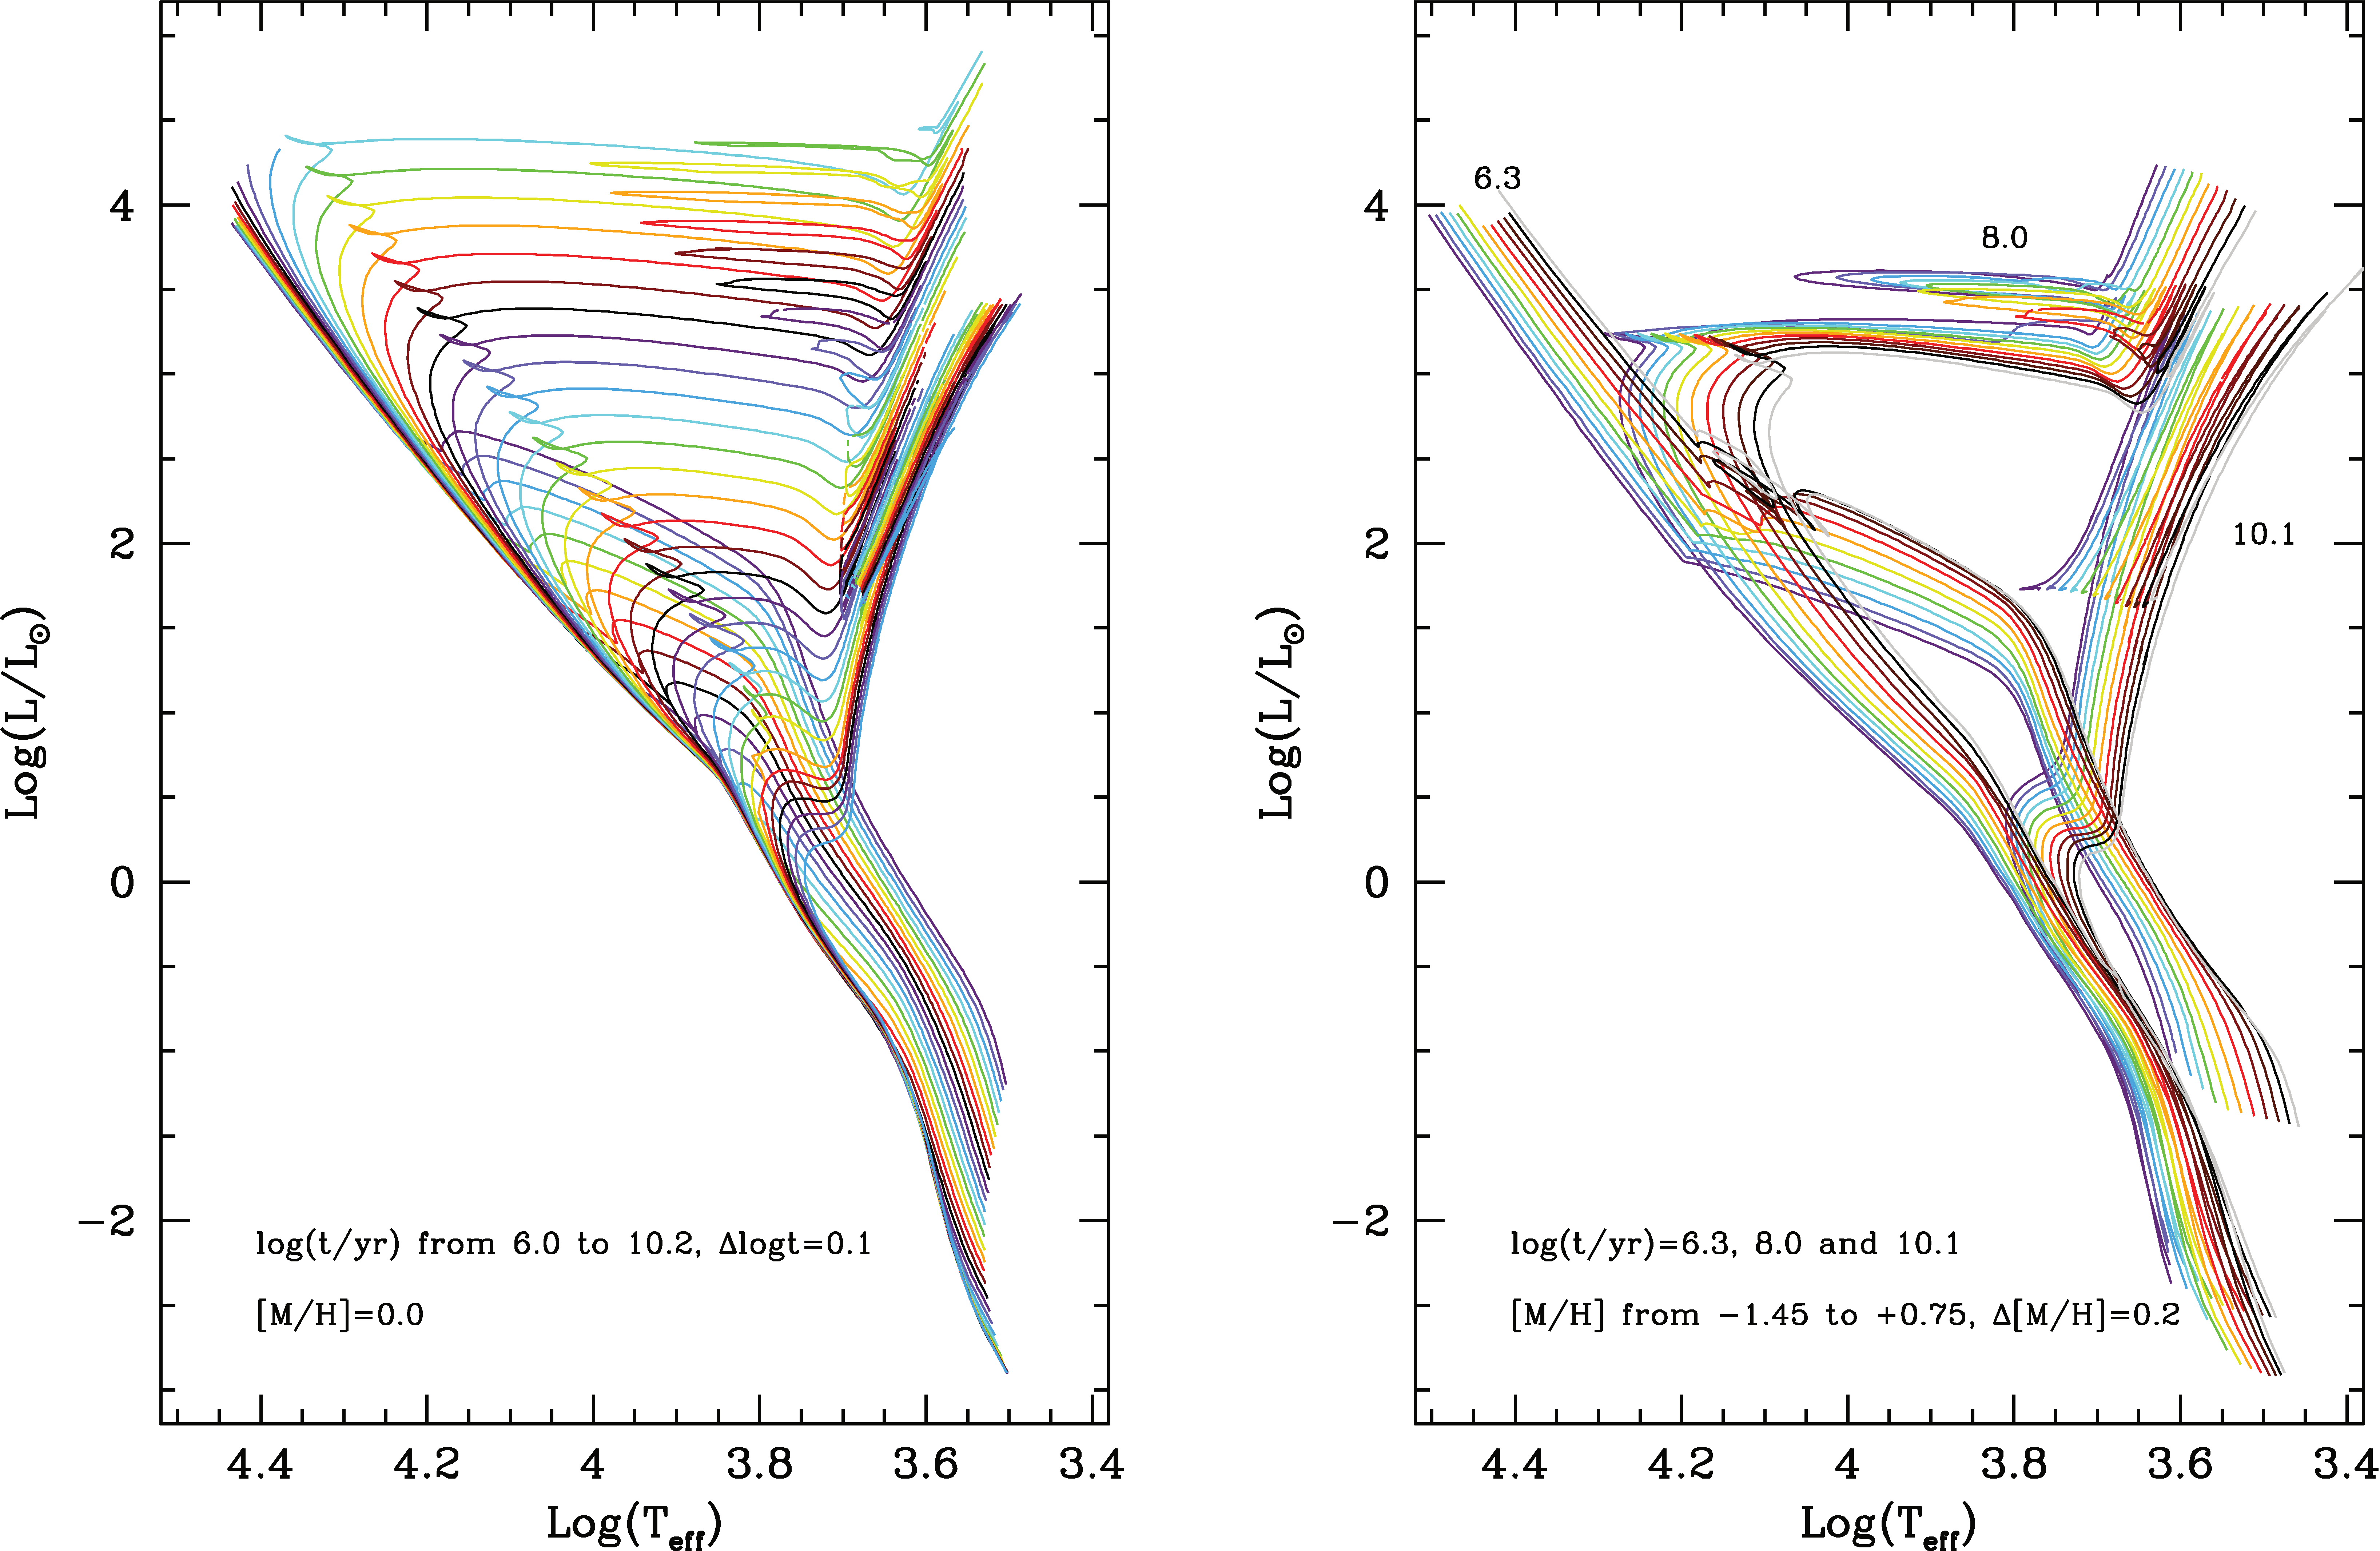
\includegraphics[width=0.9\textwidth]{../figures/theoretical_isochrones_in_hr_diagrams.pdf}
  \caption{Examples of theoretical isochrones in the HR diagram taken from \protect\citeA[p.~16]{bressan2012parsec}}
  \label{fig:examples_of_isochrones}
\end{figure}

\chapter{State of the Art}

An initial approach to find OC is the search of overdensities along the galactic disk. In general, this is the initial point,
but even it looks simple, it presents a fundamental problem. The near field around the OC is fulled by two differenciated
kind of stars populations: the ones which belong to the OC (from a tens or hundreds to a few thousand) and a background composed
by thousands or millions of stars which don't belong to the OC. Find out which stars belong to the first group is the problem
treated in this work. This selection is crucial to properly characterize the fundamental properties of the cluster
(dynamics, total mass, age, chemical composition, etc.).

Sometimes, this problem is easy to solve by looking into astrometric parameters, such as the analysis of proper motion of those
stars belonging to the overdensity field.

\begin{figure}[htbp]
  \centering
  \begin{subfigure}{0.9\textwidth}
    \centering
    \begin{subfigure}[t]{0.45\textwidth}
      \centering
      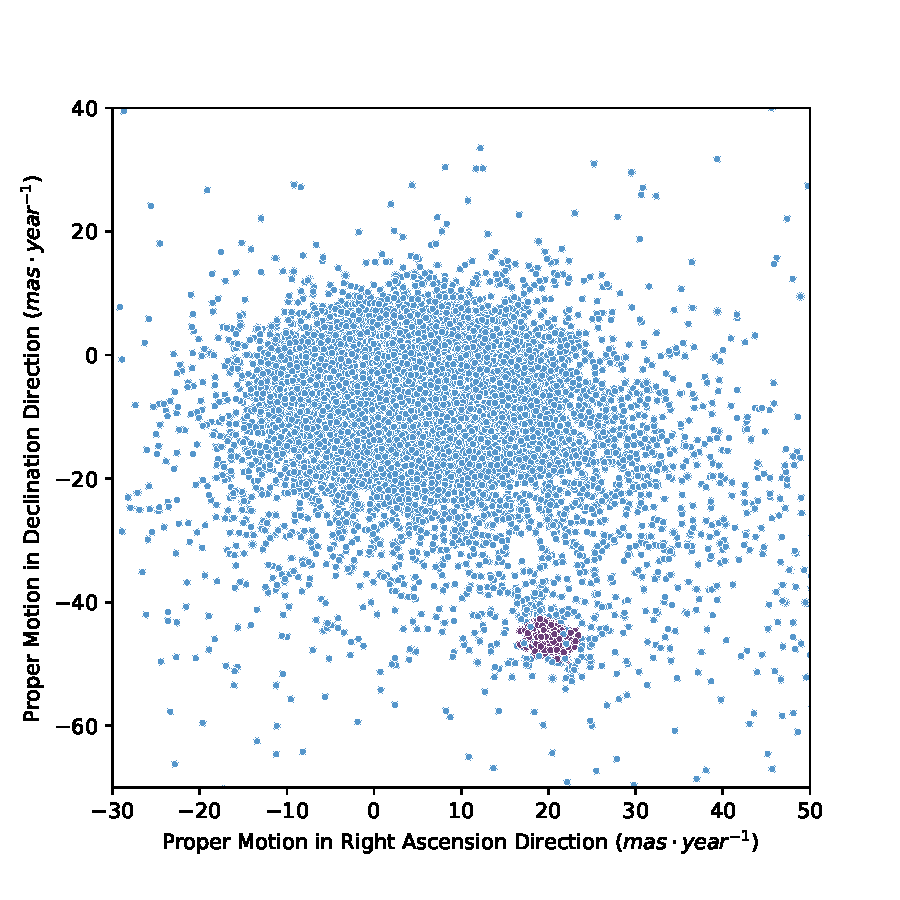
\includegraphics[width=\textwidth]{../figures/pm_melotte_22.pdf}
      \caption{Proper motions}
      \label{fig:pm_melotte_22}
    \end{subfigure}
    \hfill
    \begin{subfigure}[t]{0.45\textwidth}
      \centering
      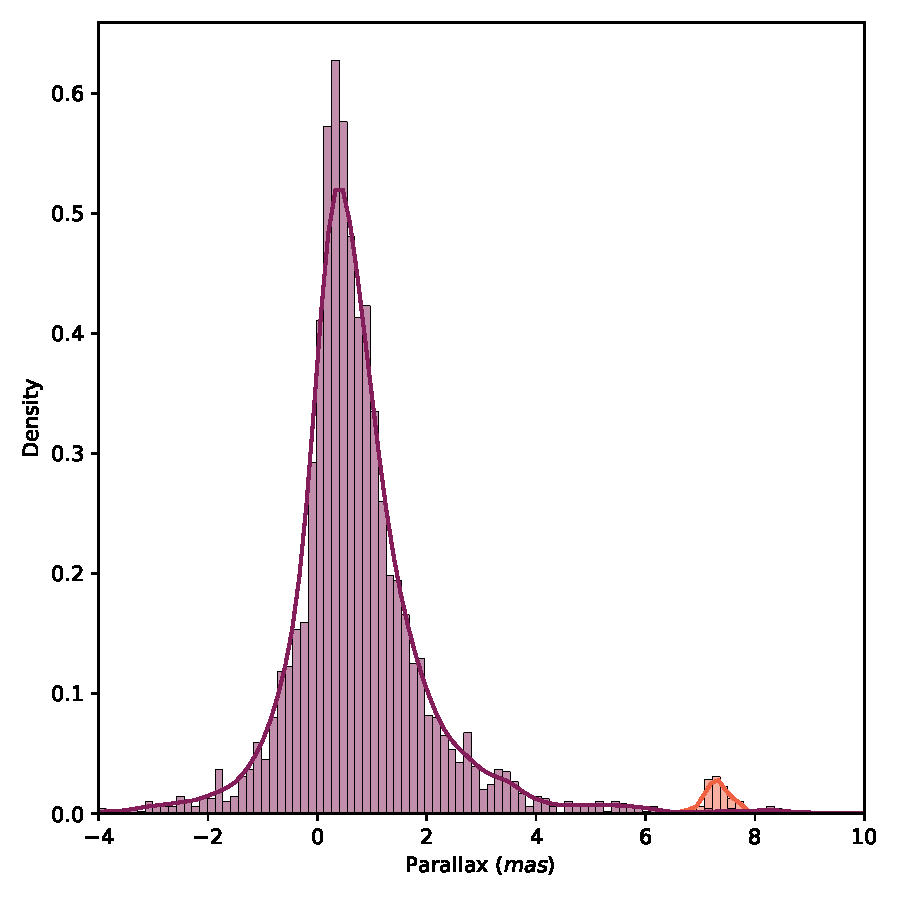
\includegraphics[width=\textwidth]{../figures/parallax_melotte_22.pdf}
      \caption{Parallax}
      \label{fig:pm_vec_melotte_22}
    \end{subfigure}
  \end{subfigure}
  \caption{Open Cluster Melotte 22 (M45)}
\end{figure}

Figure \ref{fig:pm_melotte_22} shows the proper motion distribution in right ascension and declination.
It is easy to see that a subgroup can be located at [20, -45].
Figure \ref{fig:pm_vec_melotte_22} shows the parallax density and confirms an overdensity at $\approx 7.5 mas$ corresponding to Mellote 22 OC.

However, as shown in Figures \ref{fig:pm_ngc_6494} and \ref{fig:parallax_ngc_6494}, in general it is not as easy and
becomes necessary to consider other parameters such as distances, or even metallicity and age (derived from isochrone curves)
and requires photometric data from stars in the studied field
\footnote{All figures have been sampled in order to reduce the document size, but are still a faithful representation of the original data}.

\begin{figure}[htbp]
  \centering
  \begin{subfigure}{0.9\textwidth}
    \centering
    \begin{subfigure}[t]{0.45\textwidth}
      \centering
      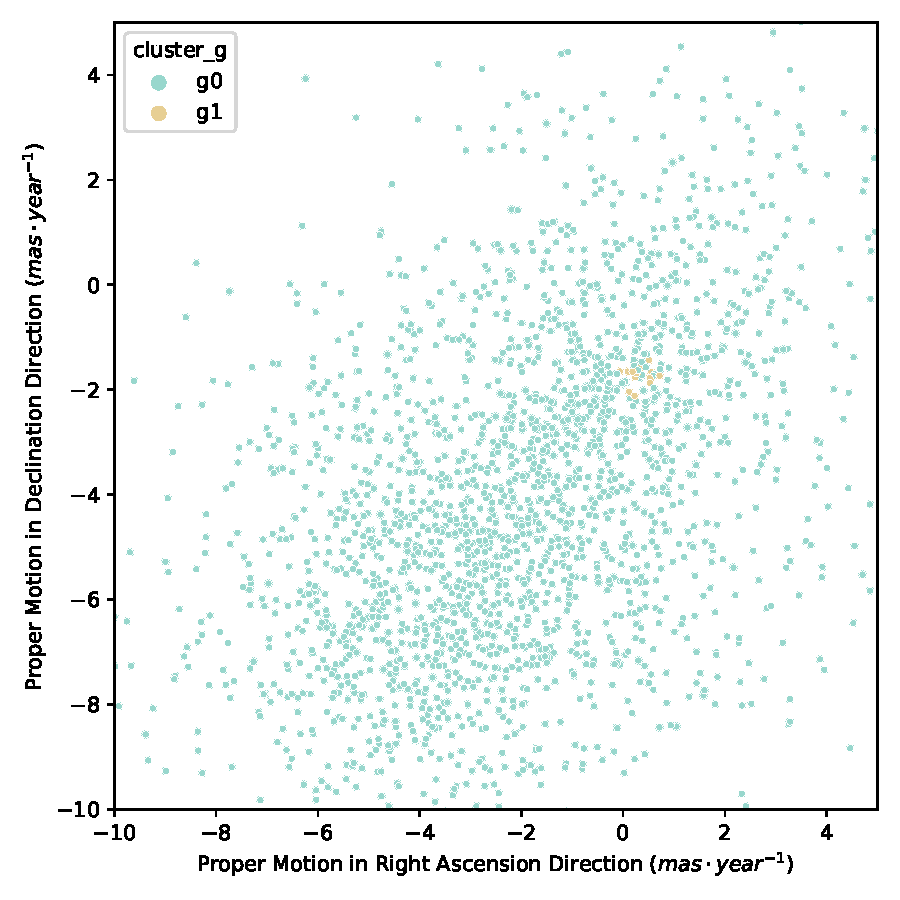
\includegraphics[width=\textwidth]{../figures/pm_ngc_6494.pdf}
      \caption{Proper motions}
      \label{fig:pm_ngc_6494}
    \end{subfigure}
    \hfill
    \begin{subfigure}[t]{0.45\textwidth}
      \centering
      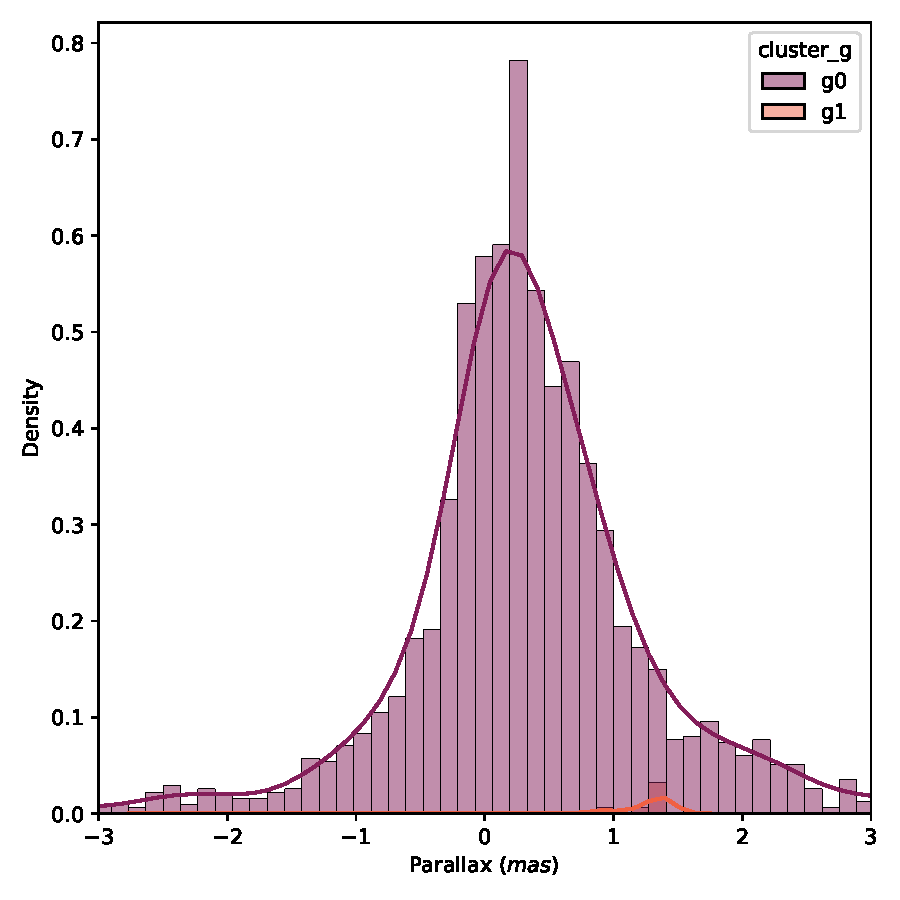
\includegraphics[width=\textwidth]{../figures/parallax_ngc_6494.pdf}
      \caption{Parallax}
      \label{fig:parallax_ngc_6494}
    \end{subfigure}
  \end{subfigure}
  \caption{Open Cluster NGC 6494}
\end{figure}

At this point, it looks reasonable that the study of each individual cluster requires its own parametrization and technique
to identify it.

With Gaia DR2, which contains great quality astrometrical and photometric data for a huge number of stars,
a new opportunity to simplify and optimize this processes is presented.
In this context new approaches are being developed to improve current detection methods and automate the OC characterization.
This work tries to take the best from \emph{Clusterix 2.0. A Virtual Observatory tool to estimate cluster membership probability}
\cite{balaguer2020clusterix} and \emph{Hunting for open clusters in Gaia DR2: 582 new open clusters
in the Galactic disc} \cite{castro2020hunting}, and merge them into a single \emph{machine learning}
tool capable of finding open clusters eficiently without requiring powerful machines to perform the computations.

The first one is a non-parametrized method. It determines empirically the frequency functions asociated to astrometrical variables
without making any assumption about their profiles. However, it heavily does depend on the initial field selection and other
parameters related to frequency functions. \emph{Clusterix 2.0.} is a web app tool inside the Spanish Virtual Observatory
(VO) framework and works together with other VO tool such as:
\emph{TOPCAT} \cite{taylor2005topcat},
\emph{Aladin} \cite{bonnarel2000aladin},
\emph{VOSA} \cite{bayo2008vosa}, among other.

The second tool is based on Big Data techniques. Its purpose is to analyze the whole Gaia DR2 dataset looking for OCs by using
machine learning algorithms divided in two stages. In the first stage, the algorithm looks for posible OC candidates by searching
overdensities in the galactic disc.
The second stage studies candidates found in the first one by generating images with H-R diagrams and passing them
as sources to an Artificial Neural Network (ANN) which identifies isochrone patterns in photometric data (color and magnitude).
Before this approach was put into practice there were 1200 OCs known. Now, this number has been increased up to more than 2000 OCs
available at the Vizier catalogue \cite{ochsenbein2000vizier}.

The method developed in this project takes as base the approach made by \citeauthor{castro2020hunting} but rapidly diverges.
In first place, performance has been taken into account since the begining, trying to get a reliable method without compromising the
needs of supercomputers.
To achieve this, instead of blindly analyzing the whole galactic disk a fields selection is made focusing in those regions with known OCs.
Then, these fields are analyzed with an homogeneous methodology based on machine learning algorithms using as sources astrometric and
photometric variables. The goal is the characterization of each individual star in the cluster, discerning wether the star belongs the OC
or not.

Thus, the main goal of this project is not the discovery of new open clusters or even candidates, but the development of a model that,
applied to already knonw open clusters, allows us the characterization of those OCs on an unsupervised way, with a reasonable computing
power and taking into account the same selection of astrometric and photometric variables for every OC.

% TODO: Hablar sobre los algoritmos de clustering que se van a emplear: K-Means, DEC

% TODO: Concluir con una última sección de resumen de conclusiones, resumiendo las principales averiguaciones del estudio del dominio
% y cómo van a afectar al desarrollo específico del trabajo.

\chapter{Aims}

\section{General}

The main aim of this thesis is to \emph{build an unsupervised clustering model for open cluster characterization}.

We want this model to be \emph{non-supervised non-parameterized} in order to fit a wide range of clusters without
the need of fine tunning hyperparameters regarding the topology or size of the studied clusters.

To measure the reliability of the resulting model comparisons with other VO tools will be made.

The role for the ANN will be validating cluster members based on dynamincs data.

These are te variables to be considered in this work:

\begin{itemize}
  \item OCs and stars \emph{right ascension}: $\alpha$ and \emph{declination}: $\delta$
  \item OCs \emph{estimated sizes}: $r$
  \item \emph{Proper motion}: $\mu_{\alpha}$, $\mu_{\delta}$ and \emph{parallax}: $\varpi$
  \item \emph{Associated errors} will be taken into account to estimate prediction errors
\end{itemize}

\section{Specific}

To achive this goal, the aim will be divided into the following milestones:

\begin{itemize}
  \item To recover data from Gaia DR2 database. This data will be taken as source for the machine learning model to characterize open clusters
  by grouping stars into clusters.
  \item To research unsupervised clustering algorithms suitable for grouping stars previously recovered.
  \item To select and implement unsupervised clustering algorithms from the previous study.
  \item To apply implemented tools to different datasets from first point to find OCs.
  \item To validate found OCs by determining their accuracy and precission.
\end{itemize}

% TODO: Hay que desarrollar más los objetivos

\chapter{Method}

In this chapter we address the different steps taken to perform the creation of the unsupervised clustering model for open cluster characterization.

All code is developed with the Python programming language \cite{Python3}. Other auxiliary tools such as \emph{Docker} \cite{merkel2014docker},
\emph{PostgreSQL} \cite{postgresql}, \emph{Jupyter Notebooks} \cite{Kluyver2016jupyter}, and \emph{Astropy} \cite{astropy:2013} \cite{astropy:2018},
\emph{Scikit-Learn} \cite{scikit-learn}, \emph{seaborn} \cite{michael_waskom_2017_883859}, \emph{SQLAlchemy} \cite{sqlalchemy} and
\emph{Keras} \cite{chollet2015keras} frameworks have been used too.

\section{Data Mining}

As mentioned before, I have chosen the Gaia DR2 database as the data source for this work. Thus, the first step is to download the required data from Gaia DB
and store it in a custom database for later access.

Due to the large amount of data inside Gaia database, a complete download is not viable neither useful.
In order to squize the size of the dataset to be downloaded, the OpenClust catalogue \cite{dias2002new} (Figure \ref{fig:OpenClustComplete})
has been used to make a preselection of sky regions.

This download is not limited to the size registered in the catalogue. Instead, a wider region is downloaded for each cluster to include
stars outside the cluster and take them into account when training the model so the model will be able to take apart those outsiders
when characterizing the cluster.

\begin{figure}[htbp]
  \centering
  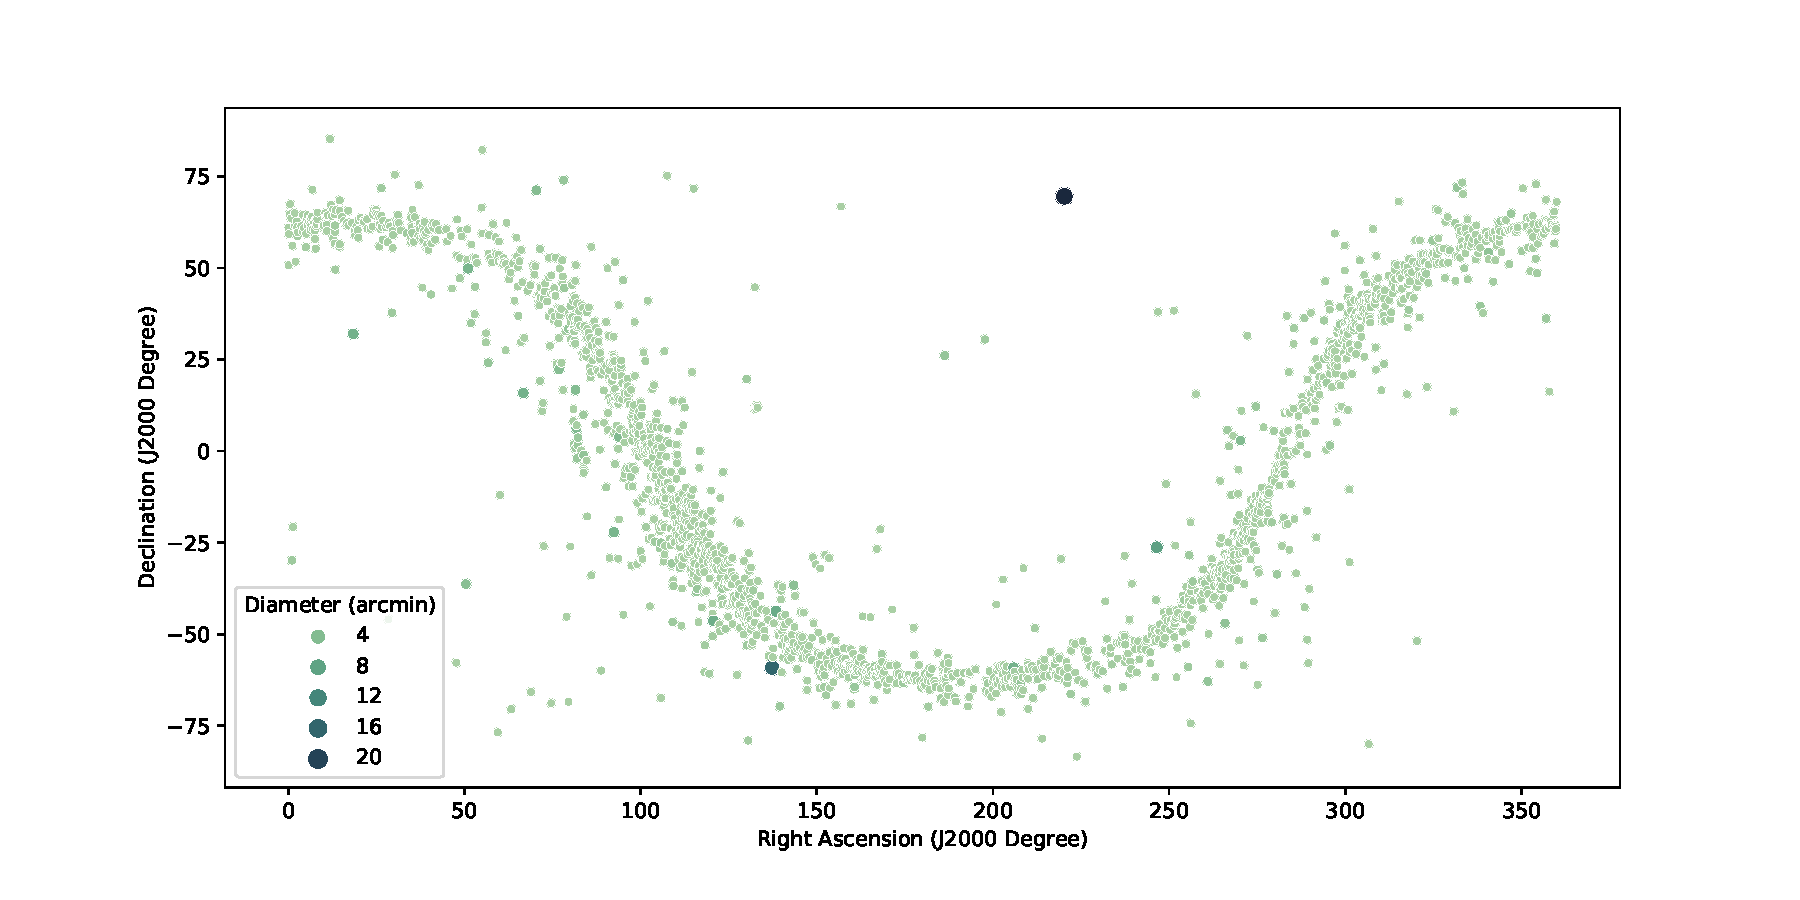
\includegraphics[width=0.9\textwidth]{../figures/openclust_catalogue.pdf}
  \caption{OpenClust Catalogue Distribution}
  \label{fig:OpenClustComplete}
\end{figure}

The downloaded dataset covers nearly 114 million stars (42GB of compressed data), that is significantly smaller than the whole Gaia DR2 dataset, which contains
information for around 1,600 million stars, but stils being too large.

Since not all the downloaded clusters are good enough, the following filters are applied to discard some clusters which don't have enough stars or contain too
many \emph{null} values:

\begin{itemize}
  \item Cluster diameter above 25.0 arcmin
  \item Parallax absolute value greater than 0.0
  \item Number of stars in the selected region above 40,000 stars
\end{itemize}

As shown in Figure \ref{fig:OpenClustSelection} this selection stills being a good representation of all clusters in the Milky Way since they are
equally distributed around the galaxy line.

After this selection, the number of cluster to look up is 169 with nearly 75 million stars.

Since there is no upper limit to the number of stars inside a cluster, for the sake of simplicity and as a commitment to the project delivery dates
and the available computing power, smaller clusters will be prefered over the greatest ones.

As an extension of this work, the designed model could be applied to a region not covered by this preselection for a later understanding of the results.

\begin{figure}[htbp]
  \centering
  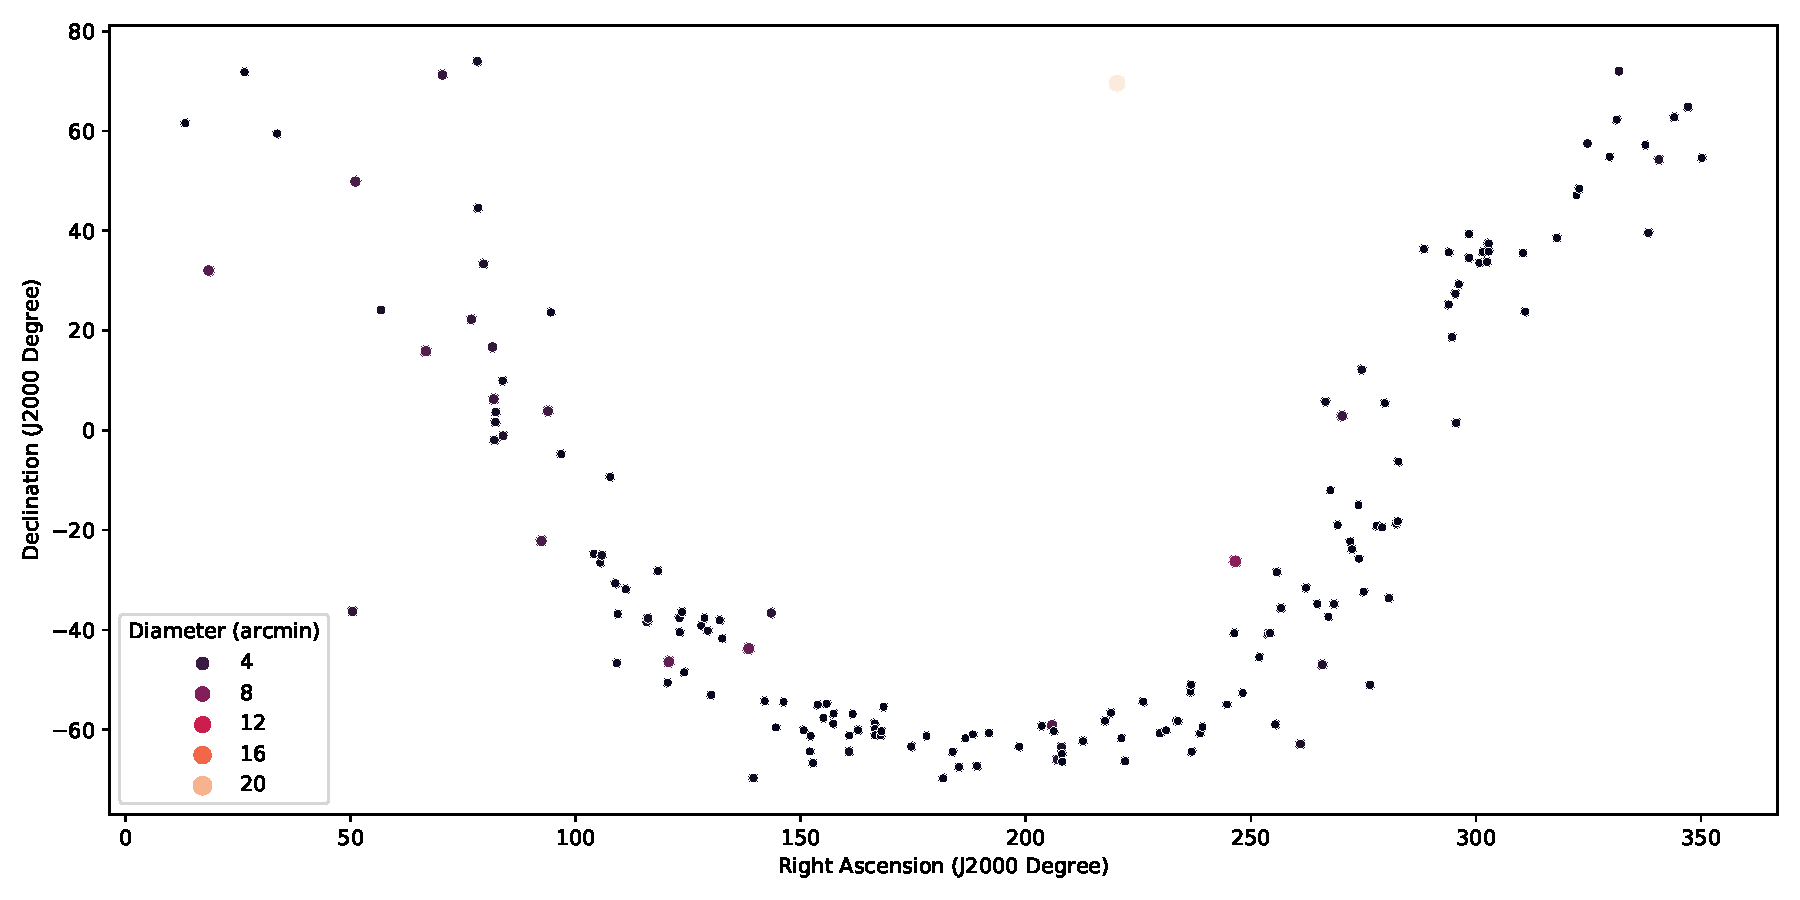
\includegraphics[width=0.9\textwidth]{../figures/cluster_selection_tier1.pdf}
  \caption{OpenClust Catalogue Selection Distribution}
  \label{fig:OpenClustSelection}
\end{figure}

The download process has been performed with two Docker containers: a \emph{downloader} and the \emph{database}.

The first one is a container built from a \verb|python:3.8| image that contains the \verb|cdalvaro| package and the \verb|downloader.py| script.
This script is prepared to load the OpenClust catalogue, connect to the Gaia DR2 database, download all stars contained inside each cluster
(with a radius multiplier to increse the area to be downloaded) and save the downloaded data inside the custom database hosted in the second container.

Downloader image build instructions are available at \href{https://github.com/cdalvaro/machine-learning-master-thesis/blob/main/src/downloader.Dockerfile}{downloader.Dockerfile}
and latest image is available for pulling from \href{https://github.blog/2020-09-01-introducing-github-container-registry/}{GitHub Container Registry}:

\begin{minted}{sh}
  docker pull ghcr.io/cdalvaro/gaia-downloader:latest
\end{minted}

This image is automatically built with \href{https://github.com/features/actions}{GitHub Actions} on every push to the \verb|main| branch.

The second container is just a \verb|postgres:12.4| image which loads an initial script when the database is not yet initialized for creating the
database schema. This container is used later as the main database for data analysis.

The database has two main tables, \verb|regions| for storing cluster properties such as location, diameter and other properties, and \verb|gaiadr2_source|
which contains data for all downloaded stars. This second table is partitioned by region, storing all stars related to one cluster inside an independent
table for faster access.

Methods for retrieving information from the database are available through an instance of \verb|cdalvaro.DB|. This class contains methods
for recovering stars information for a given region as a Pandas \verb|DataFrame| ready for data analysis.

These containers are orchestrated with a \href{https://github.com/cdalvaro/machine-learning-master-thesis/blob/main/src/docker-compose.yml}{docker-compose.yml}
file which automatilly launches one instance of each container.

The code developed for this work can be found inside the \verb|src| directory at GitHub:
\href{https://github.com/cdalvaro/machine-learning-master-thesis}{cdalvaro/machine-learning-master-thesis}

\section{Soft Clustering with K-Means}

Our first approach to find the open cluster inside the interest region is to use the K-Means algorithm.

Since we are looking for a cluster, it seems reasonable to use a clustering algorithm and set it to find two clusters.
One for the desired OC and another cluster which contains stars that don't belong to the open cluster.
However, this idea is not right.

This is due to the fact that OC's stars are sourounded by other stars with possibly similar properties. So, setting the number of clusters
to two is too low to separate them properly.

As shown in Figure \ref{fig:kmeans_comparisons_melotte_22}, bigger values for the number of clusters allow us to isolate more accurately
the resonance in parallax at $\approx 7.5mas$. However, we have the disadvantage that more groups are formed, while our aim is to find just
one small cluster and another with the rest of stars. This effect complicates our task of finding the desired OC. Thus, we have to find
the right value to isolate the searched cluster without creating to many groups.

\begin{figure}[htbp]
  \centering
  \begin{subfigure}{0.9\textwidth}
    \centering
    \begin{subfigure}[t]{0.3\textwidth}
      \centering
      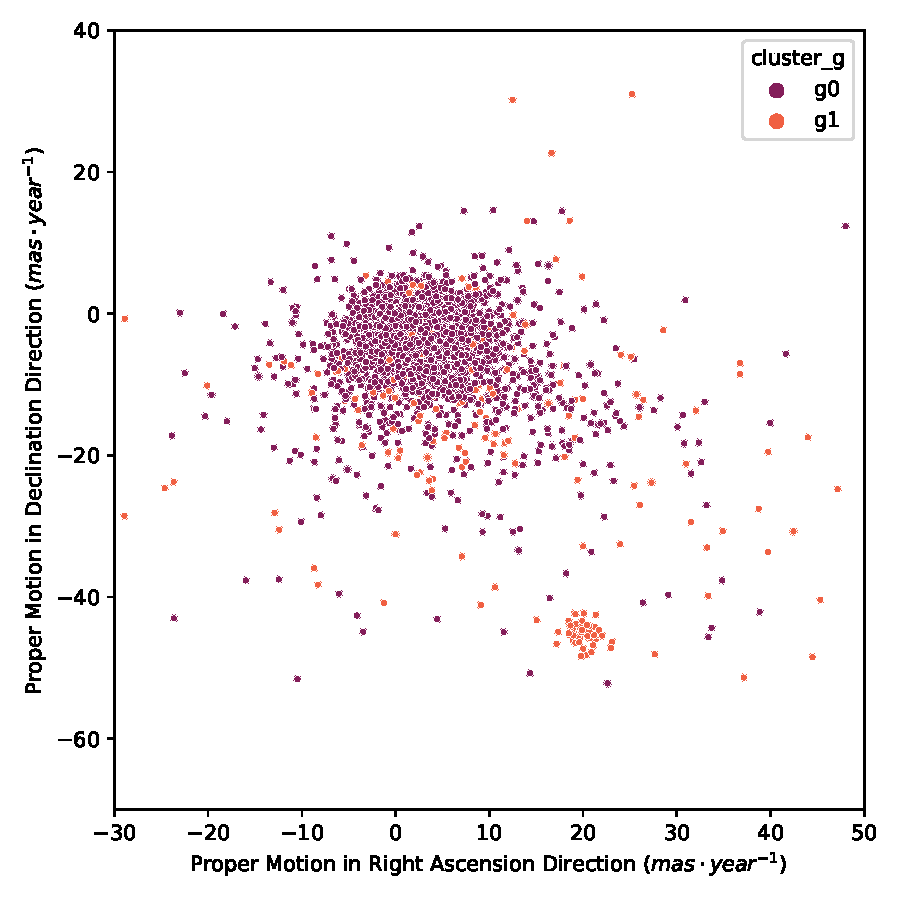
\includegraphics[width=\textwidth]{../figures/kmeans_n2_pm_melotte_22.pdf}
    \end{subfigure}
    \hfill
    \begin{subfigure}[t]{0.3\textwidth}
      \centering
      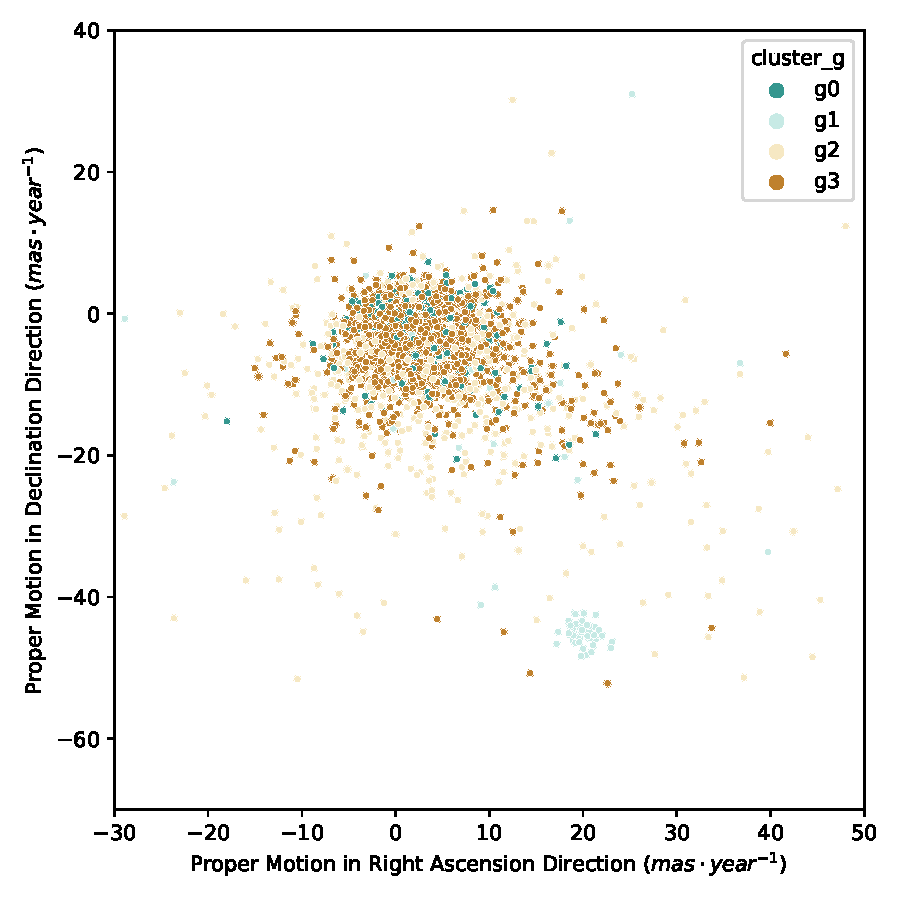
\includegraphics[width=\textwidth]{../figures/kmeans_n5_pm_melotte_22.pdf}
    \end{subfigure}
    \hfill
    \begin{subfigure}[t]{0.3\textwidth}
      \centering
      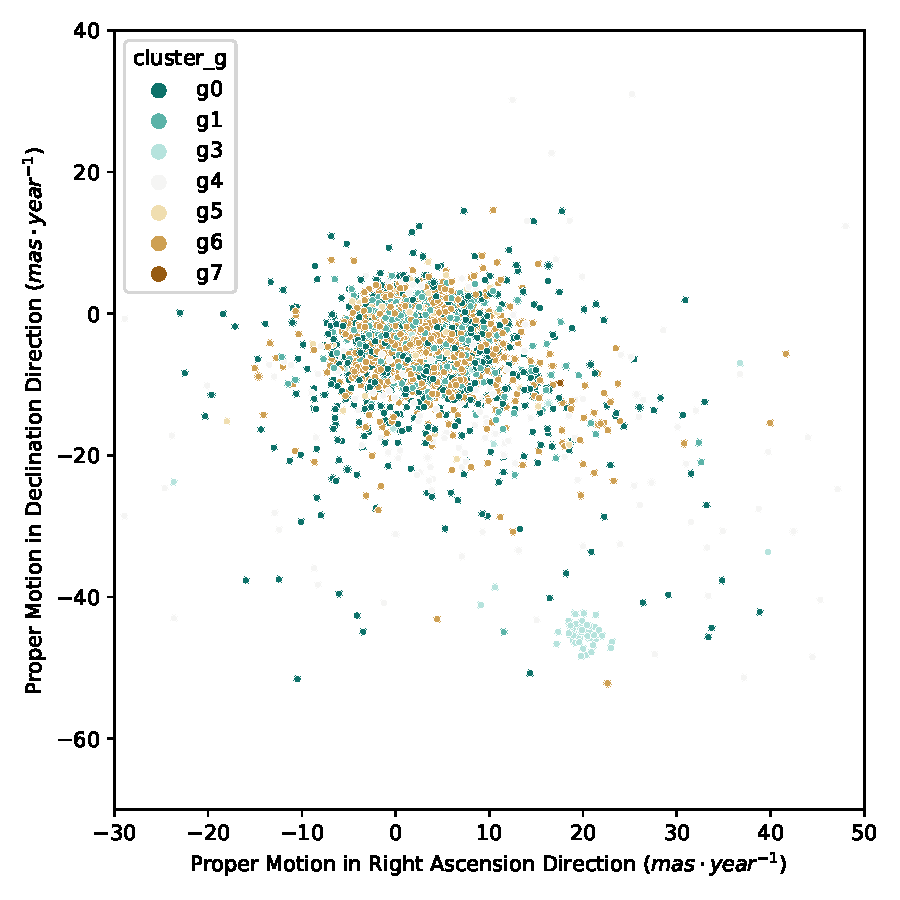
\includegraphics[width=\textwidth]{../figures/kmeans_n8_pm_melotte_22.pdf}
    \end{subfigure}
  \end{subfigure}
  \medskip
  \begin{subfigure}{0.9\textwidth}
    \centering
    \begin{subfigure}[t]{0.3\textwidth}
      \centering
      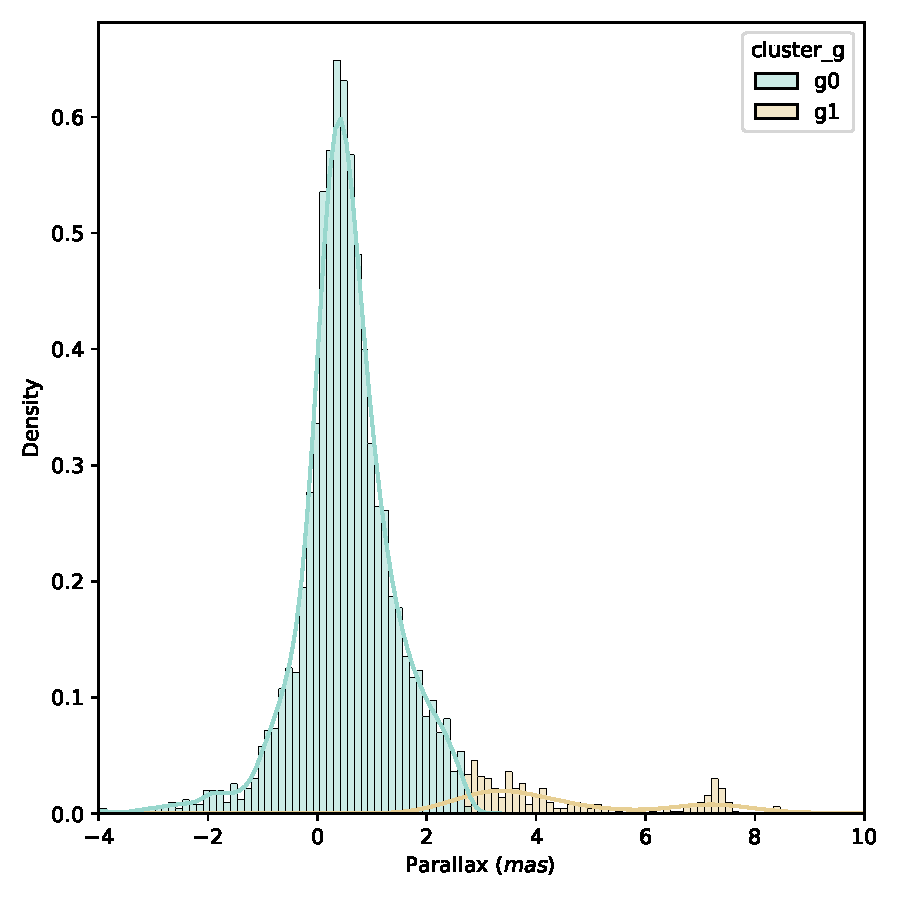
\includegraphics[width=\textwidth]{../figures/kmeans_n2_parallax_melotte_22.pdf}
      \caption{N clusters = 2}
    \end{subfigure}
    \hfill
    \begin{subfigure}[t]{0.3\textwidth}
      \centering
      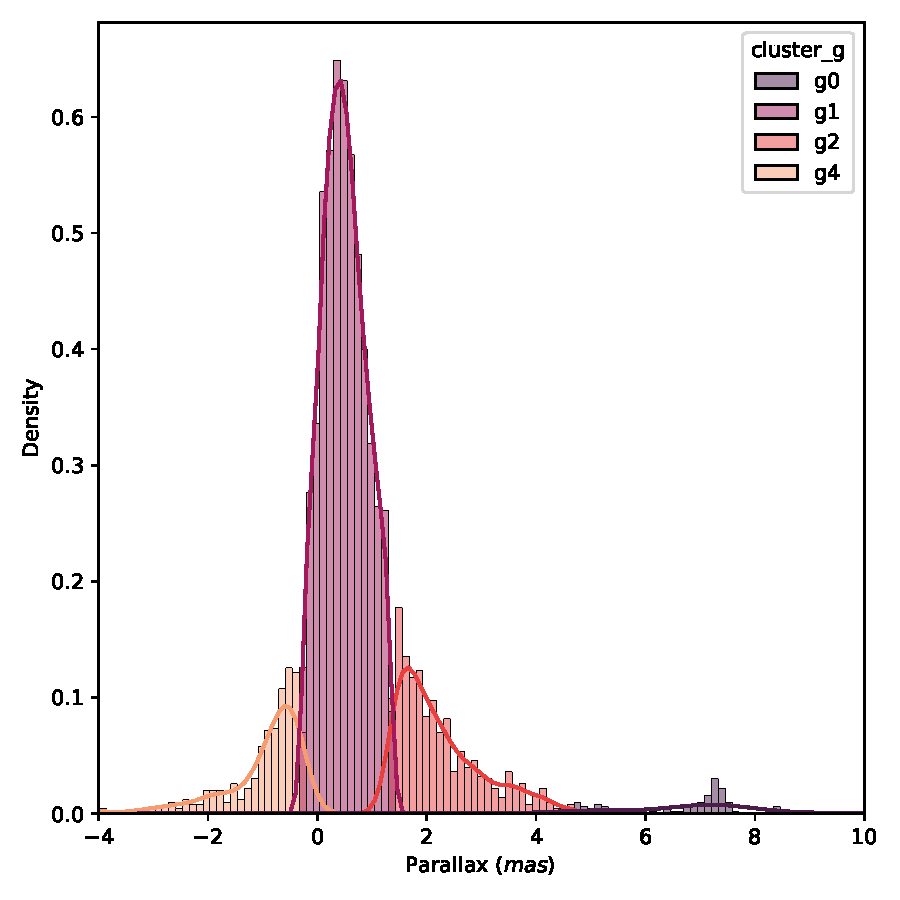
\includegraphics[width=\textwidth]{../figures/kmeans_n5_parallax_melotte_22.pdf}
      \caption{N clusters = 5}
    \end{subfigure}
    \hfill
    \begin{subfigure}[t]{0.3\textwidth}
      \centering
      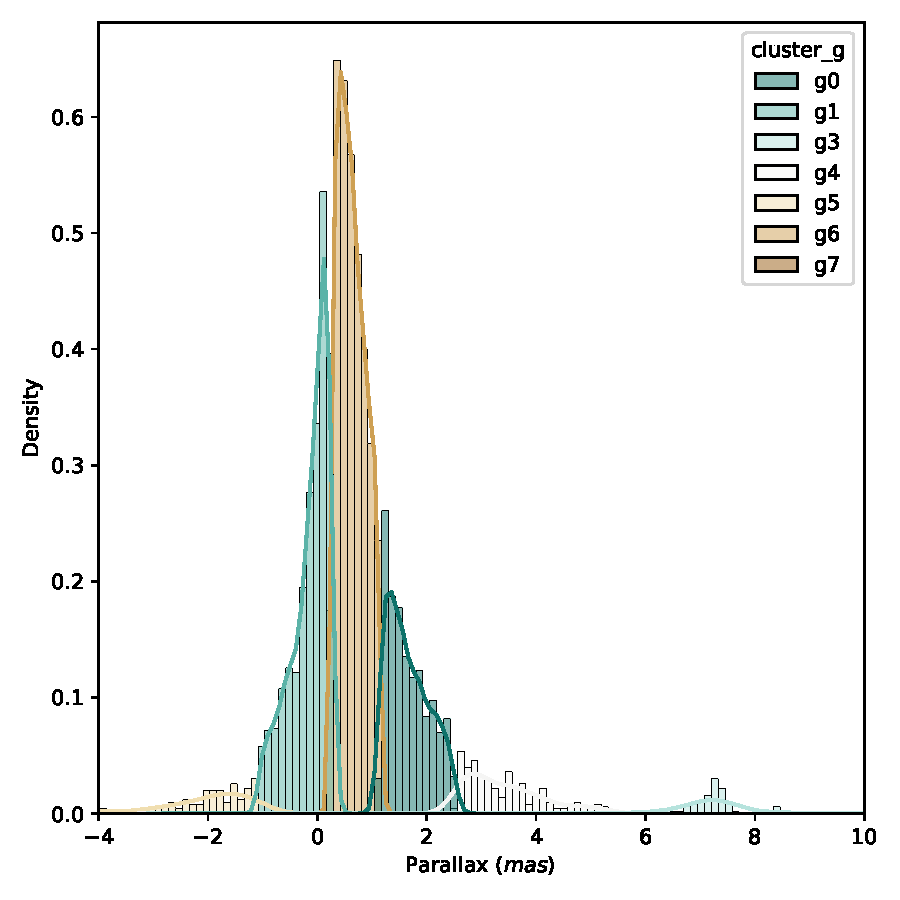
\includegraphics[width=\textwidth]{../figures/kmeans_n8_parallax_melotte_22.pdf}
      \caption{N clusters = 8}
    \end{subfigure}
  \end{subfigure}
  \caption{K-Means comparisons with Melotte 22}
  \label{fig:kmeans_comparisons_melotte_22}
\end{figure}

To solve this issue, we will try to estimate the best number of clusters by using the \emph{silhouette score}.

The silhouette score is a metric used to determine how good a cluster is based on intra-cluster distances and nearest-cluster distances.
The best possible value is 1, and the worst is -1. Negative values mean that some samples have been assigned to the wrong cluster.

\section{Deep Embedded Clustering}

Our initial approach allows us to find some groups that potentially contain the desired OC. However we need now a method for merging clusters
by migrating stars from one group to another. So we can end up with the minimum number of clusters while preserving the open cluster.

Since we don't have a labeled dataset which allows as to train a supervised model, we are required to use an unsupervised self-trained model.

For that purpose we have adapted the Unsupervised Deep Embedding for Clustering Analysis or DEC model \cite{xie2016unsupervised} to our work.

The implementation of this model is available in \verb|cdalvaro.ml.DEC| and it is developed with the Keras framework.

The model is composed by a \emph{deep autoencoder}, a \emph{deep encoder} and a \emph{clustering layer}.

Encoders are used to transform the input data into a latent space using a non-linear mapping function $f_{\theta} : X \rightarrow Z$.

Although in this work we are managing a small number of features, this latent space allows us to reduce the number of features, avoiding
this way the \emph{"curse of dimensionality"} \cite{bellman1961curse}.

These encoders are pretrained before fitting the model to generate predictions. Then, the encoder is used to transform input data to the
latent space $Z$. Once the data has been transformed, a K-Means clusterer is used to make an initial clustering of the data.

With that initial configuration, the model iterates alternating between computing an auxiliary target distribution (Soft Assignment)
and minimizing the Kullback-Leiber (KL) divergence \cite{kullback1951information} to it. This unsupervised algorithm allows us to improve
the clustering.

In the soft assignment stage, the \emph{Student's t-distribution} is used as a kernel to measure the similarity between the embedded points
and the cluster centroid. While in the KL divergence minimization the algorithm iteratively refines clusters by learning from their high
confidence assignments with the help of an auxiliary target distribution. The model is trained by matching the soft assignment to the target
distribution. The choice of this target distribution is crucial for DEC's performance. In this work we have taken the target distribution
from DEC's original paper \cite{xie2016unsupervised}, which is defined as follows:

\begin{equation}
  p_{ij} = \frac{q^{2}_{ij} / f_{j}}{\sum_{j'}q^{2}_{ij'}/f_{j'}}
\end{equation}

Inside \href{https://github.com/cdalvaro/machine-learning-master-thesis/blob/main/src/notebooks}{src/notebooks},
there is a notebook called
\href{https://github.com/cdalvaro/machine-learning-master-thesis/blob/main/src/notebooks/cluster_characterization.ipynb}{cluster\_characterization.ipynb}
that illustrates how DEC model process a region of stars trying to characterize the OC hidden inside that region.

As we can see in Figure \ref{fig:dec_melotte_22}, the DEC model is able to merge similar clusters leaving alone the OC. Which is exactly what we are looking for.

\begin{figure}[htbp]
  \centering
  \begin{subfigure}{0.9\textwidth}
    \centering
    \begin{subfigure}[t]{0.3\textwidth}
      \centering
      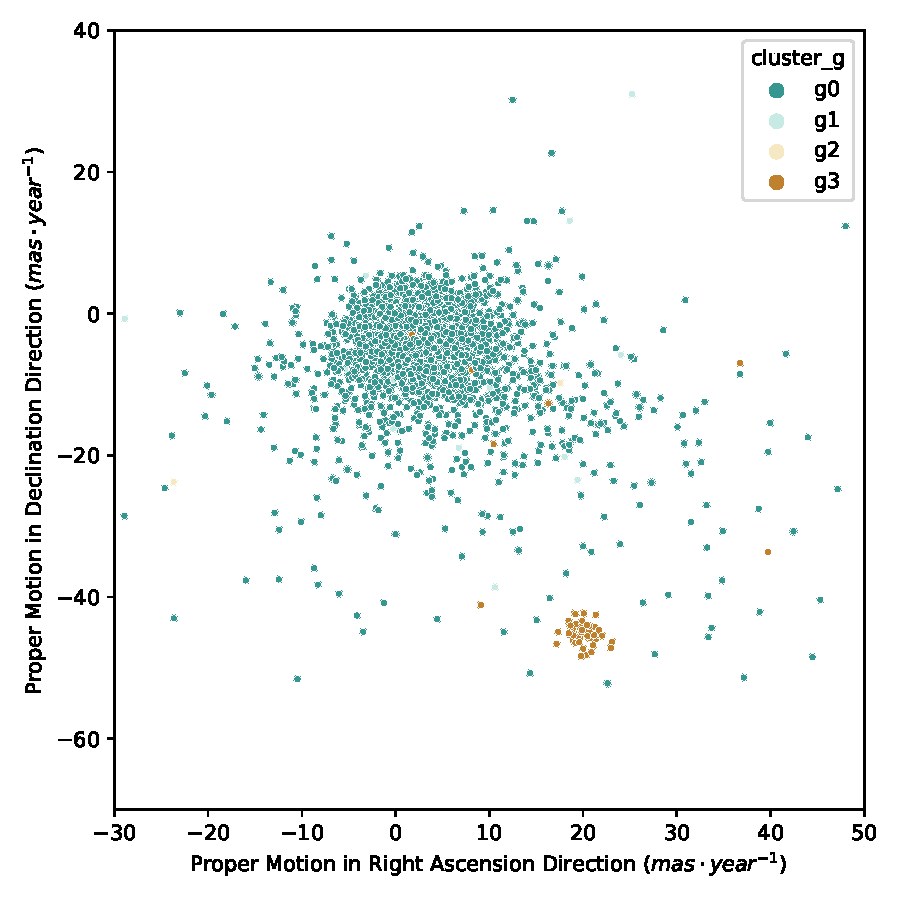
\includegraphics[width=\textwidth]{../figures/dec_pm_melotte_22.pdf}
      \caption{Proper motions}
    \end{subfigure}
    \hfill
    \begin{subfigure}[t]{0.3\textwidth}
      \centering
      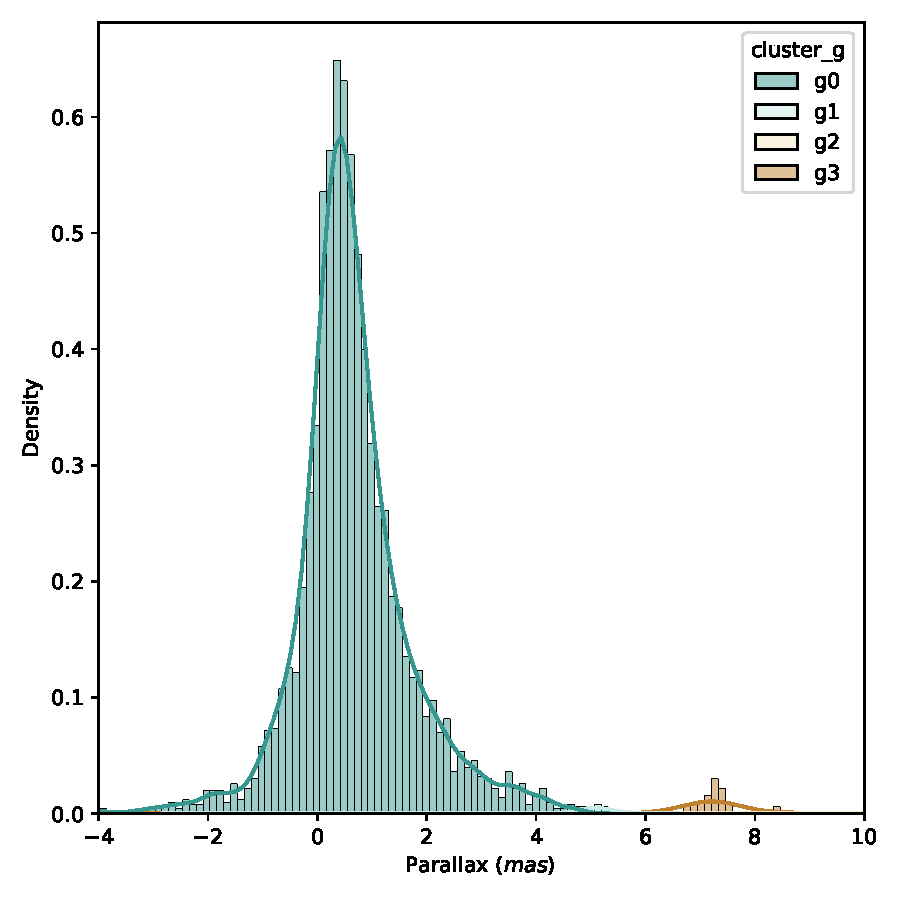
\includegraphics[width=\textwidth]{../figures/dec_parallax_melotte_22.pdf}
      \caption{Parallax}
    \end{subfigure}
    \hfill
    \begin{subfigure}[t]{0.3\textwidth}
      \centering
      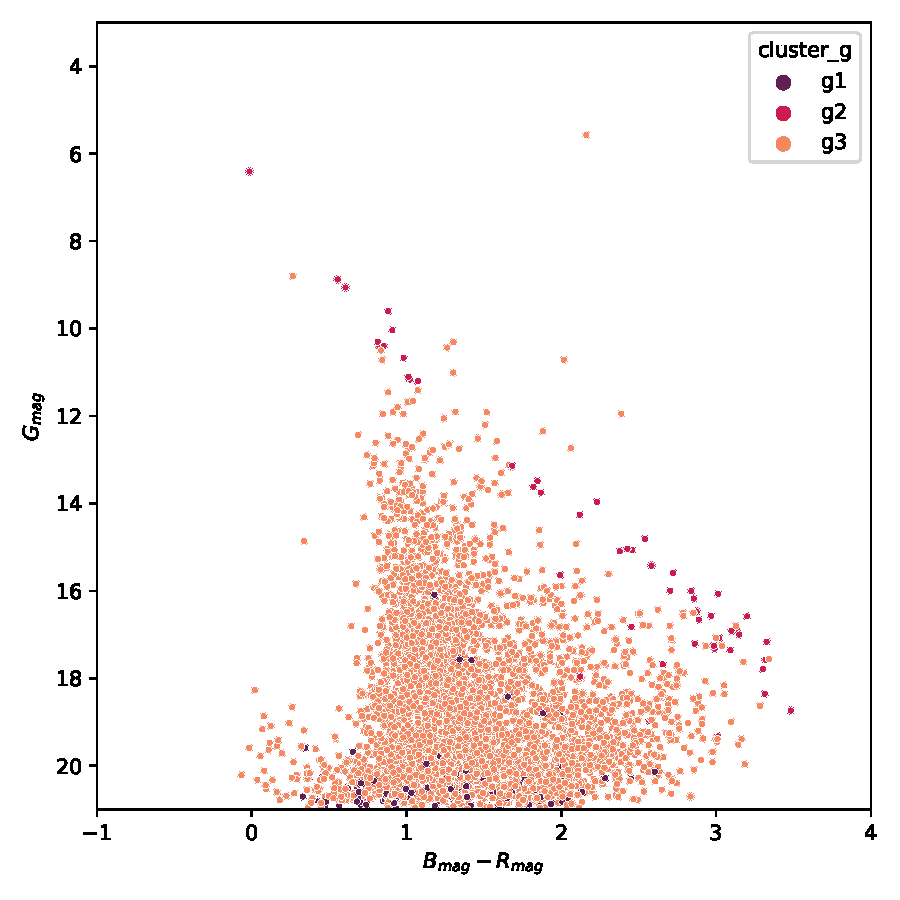
\includegraphics[width=\textwidth]{../figures/dec_isochrone_melotte_22.pdf}
      \caption{Isochrone curve}
    \end{subfigure}
  \end{subfigure}
  \caption{DEC model applied to Melotte 22}
  \label{fig:dec_melotte_22}
\end{figure}

\section{Results}

% TODO: Las tecnologías empleadas para el desarrollo de las herramientas,
% la organización del piloto, cómo ha transcurrido el experimento

% TODO: Añadir nuevo capítulo - Descripción de los resultados

% Aquí se detallan los resultados obtenidos, con tablas de resumen, gráficas de resultados, identificación de datos relevantes, etc.
% Es una exposición objetiva, sin valorar los resultados ni justificarlos.

\chapter{Discussion}

% Se aporta la discusión de los resultados presentados en el capítulo anterior. En este capítulo se puede discutir la relevancia de
% los resultados, presentar posibles explicaciones apra los datos anómalos y resaltar aquellos datos que sean parcitualarmente relevantes
% para el análisis del experimento.

\chapter{Conclusions and Future Work}

\section{Conclusions}

% Resumen final del trabajo y debe servir para informar del alcance y relevancia de la aportación.
% Suele estructurarse empezando con un resuemn del problema tratado, de cómo se ha abordado y de por qué la solución sería valída.

% Es recomendable que incluya también un resumen de las contribuciones del trabajo, en el que se relacionen las contribuciones y los
% resultado obtenidos con ls objetivos panteados para el trabajo, discutiendo hasta qué punto has conseguido resolver los objetivos planteados.

\section{Further Research}

% Debería señalar las perspectivas de futuro que abre el trabajo desarrollado para el campo de estudio definido. En el fondo,
% debe justificar de qué modo puede emplearse la aportación desarrollada y en qué campos.

\newpage

\bibliography{references}
\addcontentsline{toc}{chapter}{Bibliography}

\appendix
\chapter{Appendix}

%\includepdf[pages=-]{anexo.pdf} # TODO: Descomentar cuando el artículo esté hecho
\end{document}
